\subsection*{Objectives}

%2. La hipótesis de partida y los objetivos generales perseguidos con el proyecto coordinado en su conjunto, así como la adecuación del proyecto a la Estrategia Española de Ciencia y Tecnología y de Innovación y, en su caso, a Horizonte 2020 o a cualquier otra estrategia nacional  o internacional de 

The overall goals of this research proposal are:

\begin{enumerate}
\item Construction, commissioning and operation of the NEW and NEXT-100 detectors, during a period of 4 years, from 2015 to 2019.
\item Demonstrate the feasibility of barium tagging in an HPXe, performing a systematic set of small, focused, prove-of-concept experiments. 
\end{enumerate}
  

%%%%%%
%\begin{figure}
%\centering
%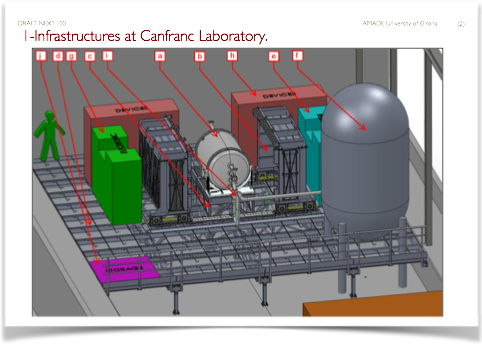
\includegraphics[width=0.9\textwidth]{img/InfraStructures.png}
%\caption{\small The infrastructures at Canfranc include: working platform, seismic pedestal, lead castle, gas system, emergency recovery system, radon suppression system and clean tent.}\label{fig.INFRA}
%\end{figure}
%%%%

%%%%%
%\begin{figure}
%\centering
%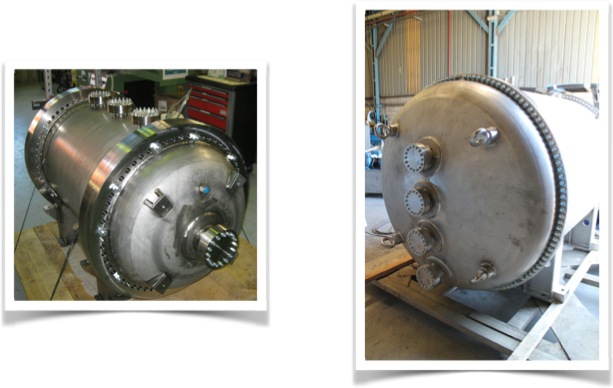
\includegraphics[width=0.9\textwidth]{img/PV.png}
%\caption{\small The NEXT pressure vessels, made of radio pure titanium-steel alloy and capable to withstand up to 25 bar pressure. Left, the NEW PV. Right, the NEXT-100 PV.}\label{fig.PV}
%\end{figure}
%%%%

%%%
\begin{enumerate}
\item {\bf Complete the needed infrastructures to operate NEW and NEXT-100 at the LSC} (Figure \ref{fig.INFRA}). The activity related with this objective has started already in 2014. The working platform, seismic pedestal and lead castle are already installed at the LSC, and the equipment related with the gas system and emergency recovery system has been purchased using AdG/ERC funds and will be installed at the LSC in the first quarter (Q1) of 2015. 

\item {\bf Complete the construction of NEW}. The current plan foresees to assemble the detector for a preliminary test at IFIC in the fourth quarter (Q4) of 2014. 
%
%After validating basic operation the detector will be disassembled. Part of the pieces (pressure vessel, copper shield, and the copper support plates of the energy plane and tracking plane) will be sent to the LSC, where they will undergo a specialised cleaning procedure designed to eliminate any traces of surface radioactivity. The field cage and the PMT enclosures (PMT ``cans'') will be sent to the Gran Sasso Underground Laboratory (LNGS), for cleaning and coating with wavelength shifters (TPB). 
The detector will be fully assembled at the LSC in the second quarter (Q2) of 2015. 
%The full construction of NEW is financed by the the AdG grant. 
 
\item {\bf Commissioning of NEW and evaluation of performance}. The detector will be brought online in Q2 2015, and extensive testing will be performed to certify safe and stable operation (no leaks, no sparks), as well as testing and integration of all the subsystems. We expect to complete commissioning in the third quarter (Q3) of 2015.
During the fourth quarter (Q4) of 2015, we will evaluate the performance of the detector. Such evaluation will allow us to correct for design problems (if they arise) or to introduce improvements in the engineering (if needed). We will also assess the overall radioactive budget of the detector, to ensure the absence of ``hot spots'' (excess of radioactivity introduced accidentally in the detector). 

\item {\bf NEW physics run}. During 2016, we will operate continuously the NEW detector at the LSC. The physics runs of NEW has several goals: a) measurement, using radioactive sources, of the energy resolution as a function of the energy, and in particular at \Qbb; b) measurement, using radioactive sources, of single (``background'') electrons, as well as ``double electrons'' (produced by the double escape peak of Tl-208, and used to characterise the signal); c) measurement of the standard mode \bbtnu; and d) a full measurement of the spectrum, after selection cuts, thus quantifying, from the data themselves, the background model. Notice that all the above measurements can be directly extrapolated to NEXT-100, since the scale between both detectors is just 1:2. 
%

\item {\bf Construction of NEXT-100}. The construction of NEXT-100 will proceed through 2015 and 2016. In fact, the pressure vessel has already been built, and other mechanical parts (inner copper shielding, and support plates) will also be built in 2015. The field cage, energy plane and tracking plane will be built in 2016, after the evaluation of performance of NEW. 

\item {\bf Commissioning of NEXT-100}. The commissioning of NEXT-100 will benefit from the experience gained commissioning and operating NEW. We consider feasible to commission the detector during the first 2 quarters of 2017, but our project management plan allows for two extra quarters. The main reason is to guarantee enough time to run with normal xenon before circulating the precious enriched xenon in the gas system and the detector. Notice that the detector can be fully calibrated, and the backgrounds can be characterised with normal xenon.  

\item {\bf Physics run of NEXT-100}. The physics run may start in the third quarter of 2017, but the project plan foresees the first quarter of 2018. After one year of run, NEXT-100 should reach the sensitivity of the current leading experiments. We currently foresee to run for three years (2018 to 2020), achieving a sensitivity to \mbb\ that makes a discovery possible if NME are sufficiently large and the neutrino is a Majorana particle. 

\item { \BATA\ \bf R\&D}: The development of the project indicates that NEXT could be upgraded to the ton scale, and its performance boosted using barium tagging. From 2014 to 2018, we aim to demonstrate the feasibility of the technology, performing a systematic set of small, prove-of-concept experiments. 
\end{enumerate}

The COORD subproject leads objective 1 (completion of infrastructures),
objective 3 (commissioning of NEW), and objective 6 (commissioning of NEXT-100). It co-leads, together with the ENG subproject objective 2 (NEW construction) and objective 5(construction of NEXT-100). It co-leads objectives 3 4, 6 and 7 (commissioning and physics run) together with CALREC and co-leads objective 8 (\BATA\ R\&D) together with CLPU.

The ENG subproject leads the development of the electronics of the NEW and NEXT-100 detector (objectives 2 and 5). Evaluation of the detector performance and physics run requires both an extensive calibration and a well tuned reconstruction, areas lead by the CALREC subproject. All the sub projects will participate in the \BATA\ R\&D. CLPU will bring in the laser technology, COORD the construction of the prototype chambers, ENG the deployment of sensors and electronics and CALREC the reconstruction of events. The participation of CLPU (BATA subproject) is essential for this objective.

%This project will allow us to complete the second and third phases of the NEXT experiment, with the construction and operation of NEW and NEXT-100.  It is important to remark that NEXT is the only large experiment in particle physics fully carried out in Spain. NEXT makes full use of the LSC facilities, boosting also its international relevance.  NEXT is a CERN recognised experiment and has been listed by NSA\footnote{http://science.energy.gov/~/media/np/nsac/pdf/docs/2014/NLDBD\_Report\_2014\_Final.pdf} as one of the key \bbonu\ experiments in the field, and the one with best future prospects. It has been supported by a CONSOLIDER-INGENIO. It brings a major contribution to the spanish program for science, including the possibility of making or participating in a fundamental discovery. The support of the AdG/ERC makes it clear that the projects suits perfectly well the goals of H2020.
